\documentclass[10pt, french]{article}
%% -----------------------------
%% Préambule
%% -----------------------------
% !TEX encoding = UTF-8 Unicode
% LaTeX Preamble for all cheatsheets
% Author : Gabriel Crépeault-Cauchon

% HOW-TO : copy-paste this file in the same directory as your .tex file, and add in your preamble the next command right after you have specified your documentclass : 
% \input{preamble-cheatsht.tex}
% ---------------------------------------------
% ---------------------------------------------

% Extra note : this preamble creates document that are meant to be used inside the multicols environment. See the documentation on internet for further information.

%% -----------------------------
%% Encoding packages
%% -----------------------------
\usepackage[utf8]{inputenc}
\usepackage[T1]{fontenc}
\usepackage{babel}
\usepackage{lmodern}

%% -----------------------------
%% Variable definition
%% -----------------------------
\def\auteur{Gabriel Crépeault-Cauchon / Nicholas Langevin}
\def\BackgroundColor{white}

%% -----------------------------
%% Margin and layout
%% -----------------------------
% Determine the margin for cheatsheet
\usepackage[landscape, hmargin=1cm, vmargin=1.7cm]{geometry}
\usepackage{multicol}

% Remove automatic indentation after section/subsection title.
\setlength{\parindent}{0cm}

% Save space in cheatsheet by removing space between align environment and normal text.
\usepackage{etoolbox}
\newcommand{\zerodisplayskips}{%
  \setlength{\abovedisplayskip}{0pt}%
  \setlength{\belowdisplayskip}{0pt}%
  \setlength{\abovedisplayshortskip}{0pt}%
  \setlength{\belowdisplayshortskip}{0pt}}
\appto{\normalsize}{\zerodisplayskips}
\appto{\small}{\zerodisplayskips}
\appto{\footnotesize}{\zerodisplayskips}

%% -----------------------------
%% URL and links
%% -----------------------------
\usepackage{hyperref}
\hypersetup{colorlinks = true, urlcolor = gray!70!white, linkcolor = black}

%% -----------------------------
%% Document policy (uncomment only one)
%% -----------------------------
%	\usepackage{concrete}
	\usepackage{mathpazo}
%	\usepackage{frcursive} %% permet d'écrire en lettres attachées
%	\usepackage{aeguill}
%	\usepackage{mathptmx}
%	\usepackage{fourier} 

%% -----------------------------
%% Math configuration
%% -----------------------------
\usepackage[fleqn]{amsmath}
\usepackage{amsthm,amssymb,latexsym,amsfonts}
\usepackage{empheq}
\usepackage{numprint}
\usepackage{dsfont} % Pour avoir le symbole du domaine Z

% Mathematics shortcuts

\newcommand{\reels}{\mathbb{R}}
\newcommand{\entiers}{\mathbb{Z}}
\newcommand{\naturels}{\mathbb{N}}
\newcommand{\eval}{\biggr \rvert}
\usepackage{cancel}
\newcommand{\derivee}[1]{\frac{\partial}{\partial #1}}
\newcommand{\prob}[1]{\Pr \left( #1 \right)}
\newcommand{\esp}[1]{\mathrm{E} \left[ #1 \right]} % espérance
\newcommand{\variance}[1]{\mathrm{Var} \left( #1   \right)}
\newcommand{\covar}[1]{\mathrm{Cov} \left( #1   \right)}
\newcommand{\laplace}{\mathcal{L}}
\newcommand{\deriv}[2][]{\frac{\partial^{#1}}{\partial #2^{#1}}}
\newcommand{\e}[1]{\mathrm{e}^{#1}}
\newcommand{\te}[1]{\text{exp}\left\{#1\right\}}
\DeclareMathSymbol{\shortminus}{\mathbin}{AMSa}{"39}



% To indicate equation number on a specific line in align environment
\newcommand\numberthis{\addtocounter{equation}{1}\tag{\theequation}}

%
% Actuarial notation packages
%
\usepackage{actuarialsymbol}
\usepackage{actuarialangle}

%
% Matrix notation for math symbols (\bm{•})
%
\usepackage{bm}
% Matrix notation variable (bold style)
\newcommand{\matr}[1]{\mathbf{#1}}



%% -----------------------------
%% tcolorbox configuration
%% -----------------------------
\usepackage[most]{tcolorbox}
\tcbuselibrary{xparse}
\tcbuselibrary{breakable}

%%
%% Coloured box "definition" for definitions
%%
\DeclareTColorBox{definition}{ o }				% #1 parameter
{
	colframe=blue!60!green,colback=blue!5!white, % color of the box
	breakable, 
	pad at break* = 0mm, 						% to split the box
	title = {#1},
	after title = {\large \hfill \faBook},
}
%%
%% Coloured box "definition2" for definitions
%%
\DeclareTColorBox{definitionNOHFILL}{ o }				% #1 parameter
{
	colframe=blue!60!green,colback=blue!5!white, % color of the box
	pad at break* = 0mm, 						% to split the box
	title = {#1},
	before title = {\faBook \quad },
	breakable
}


%%
%% Coloured box "algo" for algorithms
%%
\newtcolorbox{algo}[ 1 ]
{
	colback = blue!5!white,
	colframe = blue!75!black,
	title=#1,
	fonttitle = \bfseries,
	breakable
}
%%
%% Coloured box "conceptgen" for points adding to a concept's deifintion
%%
\newtcolorbox{conceptgen}[ 1 ]
{
	breakable,
	colback = beaublue,
	colframe = airforceblue,
	title=#1,
	fonttitle = \bfseries
}
%%
%% Coloured box "probch3" pour formules relatives au 3ème chapitre de prob
%%
\newtcolorbox{probch3}[ 1 ]
{
	colback = ruddypink,
	colframe = burgundy,
	fonttitle = \bfseries,	
	breakable,
	title=#1
}
%%
%% Coloured box "formula" for formulas
%%
\newtcolorbox{formula}[ 1 ]
{
	colback = green!5!white,
	colframe = green!70!black,
	breakable,
	fonttitle = \bfseries,
	title=#1
}
%%
%% Coloured box "formula" for formulas
%%
\DeclareTColorBox{algo2}{ o }
{
	enhanced,
	title = #1,
	colback=blue!5!white,	
	colbacktitle=blue!75!black,
	fonttitle = \bfseries,
	breakable,
	boxed title style={size=small,colframe=arsenic} ,
	attach boxed title to top center = {yshift=-3mm,yshifttext=-1mm},
}
%%
%% Coloured box "examplebox" for formulas
%%
\newtcolorbox{examplebox}[ 1 ]
{
	colback = lightmauve,
	colframe = antiquefuchsia,
	breakable,
	fonttitle = \bfseries,title=#1
}
%%
%% Coloured box "rappel" pour rappel de formules
%%
\newtcolorbox{rappel}[ 1 ]
{
	colback = ashgrey,
	colframe = arsenic,
	breakable,
	fonttitle = \bfseries,title=#1
}
%%
%% Coloured box "rappel" pour rappel de formules
%%
\DeclareTColorBox{rappel_enhanced}{ o }
{
	enhanced,
	title = #1,
	colback=ashgrey, % color of the box
%	colframe=blue(pigment),
%	colframe=arsenic,	
	colbacktitle=arsenic,
	fonttitle = \bfseries,
	breakable,
	boxed title style={size=small,colframe=arsenic} ,
	attach boxed title to top center = {yshift=-3mm,yshifttext=-1mm},
}
%%
%% Coloured box "notation" for notation and terminology
%%
\DeclareTColorBox{distributions}{ o }			% #1 parameter
{
	enhanced,
	title = #1,
	colback=gray(x11gray), % color of the box
%	colframe=blue(pigment),
	colframe=arsenic,	
	colbacktitle=aurometalsaurus,
	fonttitle = \bfseries,
	boxed title style={size=small,colframe=arsenic} ,
	attach boxed title to top center = {yshift=-3mm,yshifttext=-1mm},
	breakable
%	left=0pt,
%  	right=0pt,
%    box align=center,
%    ams align*
%  	top=-10pt
}

%% -----------------------------
%% Graphics and pictures
%% -----------------------------
\usepackage{graphicx}
\usepackage{pict2e}
\usepackage{tikz}

%% -----------------------------
%% insert pdf pages into document
%% -----------------------------
\usepackage{pdfpages}

%% -----------------------------
%% Color configuration
%% -----------------------------
\usepackage{color, soulutf8, colortbl}


%
%	Colour definitions
%
\definecolor{blue(munsell)}{rgb}{0.0, 0.5, 0.69}
\definecolor{blue(matcha)}{rgb}{0.596, 0.819, 1.00}
\definecolor{blue(munsell)-light}{rgb}{0.5, 0.8, 0.9}
\definecolor{bleudefrance}{rgb}{0.19, 0.55, 0.91}
\definecolor{blizzardblue}{rgb}{0.67, 0.9, 0.93}
\definecolor{bondiblue}{rgb}{0.0, 0.58, 0.71}
\definecolor{blue(pigment)}{rgb}{0.2, 0.2, 0.6}
\definecolor{bluebell}{rgb}{0.64, 0.64, 0.82}
\definecolor{airforceblue}{rgb}{0.36, 0.54, 0.66}
\definecolor{beaublue}{rgb}{0.74, 0.83, 0.9}
\definecolor{cobalt}{rgb}{0.0, 0.28, 0.67}	% nice light blue-ish
\definecolor{blue_rectangle}{RGB}{83, 84, 244}		% ACT-2004
\definecolor{indigo(web)}{rgb}{0.29, 0.0, 0.51}	% purple-ish
\definecolor{antiquefuchsia}{rgb}{0.57, 0.36, 0.51}	%	pastel dark purple ish
\definecolor{darkpastelpurple}{rgb}{0.59, 0.44, 0.84}
\definecolor{gray(x11gray)}{rgb}{0.75, 0.75, 0.75}
\definecolor{aurometalsaurus}{rgb}{0.43, 0.5, 0.5}
\definecolor{ruddypink}{rgb}{0.88, 0.56, 0.59}
\definecolor{pastelred}{rgb}{1.0, 0.41, 0.38}		
\definecolor{lightmauve}{rgb}{0.86, 0.82, 1.0}
\definecolor{azure(colorwheel)}{rgb}{0.0, 0.5, 1.0}
\definecolor{darkgreen}{rgb}{0.0, 0.2, 0.13}			
\definecolor{burntorange}{rgb}{0.8, 0.33, 0.0}		
\definecolor{burntsienna}{rgb}{0.91, 0.45, 0.32}		
\definecolor{ao(english)}{rgb}{0.0, 0.5, 0.0}		% ACT-2003
\definecolor{amber(sae/ece)}{rgb}{1.0, 0.49, 0.0} 	% ACT-2004
\definecolor{green_rectangle}{RGB}{131, 176, 84}		% ACT-2004
\definecolor{red_rectangle}{RGB}{241,112,113}		% ACT-2004
\definecolor{amethyst}{rgb}{0.6, 0.4, 0.8}
\definecolor{amethyst-light}{rgb}{0.6, 0.4, 0.8}
\definecolor{ashgrey}{rgb}{0.7, 0.75, 0.71}			% dark grey-black-ish
\definecolor{arsenic}{rgb}{0.23, 0.27, 0.29}			% light green-beige-ish gray
\definecolor{amaranth}{rgb}{0.9, 0.17, 0.31}
\definecolor{brickred}{rgb}{0.8, 0.25, 0.33}
\definecolor{pastelred}{rgb}{1.0, 0.41, 0.38}

%
% Useful shortcuts for coloured text
%
\newcommand{\orange}{\textcolor{orange}}
\newcommand{\red}{\textcolor{red}}
\newcommand{\cyan}{\textcolor{cyan}}
\newcommand{\blue}{\textcolor{blue}}
\newcommand{\green}{\textcolor{green}}
\newcommand{\purple}{\textcolor{magenta}}
\newcommand{\yellow}{\textcolor{yellow}}

%% -----------------------------
%% Enumerate environment configuration
%% -----------------------------
%
% Custum enumerate & itemize Package
%
\usepackage{enumitem}
%
% French Setup for itemize function
%
\frenchbsetup{StandardItemLabels=true}
%
% Change default label for itemize
%
\renewcommand{\labelitemi}{\faAngleRight}


%% -----------------------------
%% Tabular column type configuration
%% -----------------------------
\newcolumntype{C}{>{$}c<{$}} % math-mode version of "l" column type
\newcolumntype{L}{>{$}l<{$}} % math-mode version of "l" column type
\newcolumntype{R}{>{$}r<{$}} % math-mode version of "l" column type
\newcolumntype{f}{>{\columncolor{green!20!white}}p{1cm}}
\newcolumntype{g}{>{\columncolor{green!40!white}}m{1.2cm}}
\newcolumntype{a}{>{\columncolor{red!20!white}$}p{2cm}<{$}}	% ACT-2005
% configuration to force a line break within a single cell
\usepackage{makecell}


%% -----------------------------
%% Fontawesome for special symbols
%% -----------------------------
\usepackage{fontawesome}

%% -----------------------------
%% Section Font customization
%% -----------------------------
\usepackage{sectsty}
\sectionfont{\color{\SectionColor}}
\subsectionfont{\color{\SubSectionColor}}

%% -----------------------------
%% Footer/Header Customization
%% -----------------------------
\usepackage{lastpage}
\usepackage{fancyhdr}
\pagestyle{fancy}

%
% Header
%
\fancyhead{} 	% Reset
\fancyhead[L]{Aide-mémoire pour~ \cours ~(\textbf{\sigle})}
\fancyhead[R]{\auteur}

%
% Footer
%
\fancyfoot{}		% Reset
\fancyfoot[R]{\thepage ~de~ \pageref{LastPage}}
\fancyfoot[L]{\href{https://github.com/ressources-act/Guide_de_survie_en_actuariat}{\faGithub \ ressources-act/Guide de survie en actuariat}}
%
% Page background color
%
\pagecolor{\BackgroundColor}




%% END OF PREAMBLE
% ---------------------------------------------
% ---------------------------------------------
%% -----------------------------
%% Redefine from template
%% -----------------------------
\def\auteur{Alec James van Rassel}
%% -----------------------------
%% Variable definition
%% -----------------------------
\def\cours{Apprentissage statistique en actuariat}
\def\sigle{ACT-3114}
%% -----------------------------
%% Colour setup for sections
%% -----------------------------
\def\SectionColor{green!50!black}
\def\SubSectionColor{green!20!black}
\def\SubSubSection{burntsienna}

%	"to-do" list
\newlist{todolist}{itemize}{2}
\setlist[todolist]{label=$\square$}
%% -----------------------------
%% Début du document
%% -----------------------------
\begin{document}

\begin{multicols*}{3} 

\section{Préparation de données}

\begin{algo2}[Repères visuels]
\begin{enumerate}
	\item	La \textbf{position} sur une \textbf{même échelle} (variable numérique), souvent à l’aide de points ou de boite à moustache;
	\item	La \textbf{position} sur une \textbf{échelle identique} mais \textbf{non alignée} (variable numérique);
		\begin{itemize}
		\item	Pour exemple, lorsqu’on utilise des facettes.
		\end{itemize}
	\item	La \textbf{longueur} sur une \textbf{même échelle} (variable numérique);
		\begin{itemize}
		\item	Pour exemple, dans un diagramme à bande ou un histogramme.
		\end{itemize}
	\item	L’angle ou \textbf{la pente} (variable numérique);
		\begin{itemize}
		\item	Pour exemple, en repésentant les données sous forme de lignes (pente);
		\item	Pour exemple, la redoutable pointe à tarte (angle).
		\end{itemize}
	\item	La \textbf{forme des points} (variable catégorielle) peut représenter le groupe;
	\item	L’aire ou \textbf{le volume} (variable numérique);
		\begin{itemize}
		\item	Pour exemple, dans un diagramme à bande ou un histogramme;
		\end{itemize}
	\item	La \textbf{saturation de la couleur} (numérique ou catégorielle) peut représenter “à quel point” sur une échelle de clair à foncé;
		\begin{itemize}
		\item	Pour exemple, gris vs. noir.
		\end{itemize}
	\item	La \textbf{teinte de couleur} (numérique ou catégorielle).
		\begin{itemize}
		\item	Pour exemple, bleu vs. rouge.
		\end{itemize}
\end{enumerate}
\end{algo2}

\begin{algo2}[Étapes du nettoyage de données]
Cette liste n'est pas séquentielle, il est surtout important de \textit{tout} le faire.
\begin{todolist}[leftmargin = *]
	\item	\textbf{Comprendre} la structure des données;
		\begin{itemize}
		\item	dimensions, types de variables, \texttt{str} et \texttt{summary}.
		\end{itemize}
	\item	\textbf{Visualiser} les données;
		\begin{itemize}
		\item	\texttt{head}, \texttt{summary} et graphiques exploratoires.
		\end{itemize}
	\item	\textbf{Mettre en forme \textit{(format)}} les données;
		\begin{itemize}
		\item	Chaque ligne est une observation;
		\item	Chaque colonne est une variable;
		\item	Supprimer les doublons;
		\end{itemize}
	\item	Vérifier et corriger les \textbf{types} de variables;
		\begin{itemize}
		\item	booléens, entiers, numériques, facteurs, chaines de caractères, dates, etc.
		\end{itemize}
	\item	\textbf{Manipuler} les \textbf{chaines} de caractères;
		\begin{itemize}
		\item	Corriger les typos;
		\item	Changer la casse avec \texttt{tolower};
		\item	Extraire des informations avec les expressions régulières.
		\end{itemize}
	\item	Identifier les \textbf{données aberrantes};
		\begin{itemize}
		\item	Mettre \texttt{NA} et gérer plus tard.
		\end{itemize}
	\item	\textbf{Détecter} les \textbf{erreurs} flagrantes ou les changements structurels dans les donnéesl
		\begin{itemize}
		\item	Prendre compte des réformes;
		\item	Constater les structures importantes.
		\end{itemize}
	\item	\textbf{Augmenter} les données à l'aide d'autres sources;
		\begin{itemize}
		\item	optionnel.
		\end{itemize}
\end{todolist}
\end{algo2}

\begin{conceptgen}{Types de variables}
Les jeux de données peuvent être:
\begin{description}[leftmargin = *]
	\item[Structuré:]	Données ayant une structure prédéfinie.\\
		Pour exemple:
		\begin{itemize}
		\item	Tableaux;
		\item	\og spreadsheet \fg{};
		\item	\og Relational databases \fg{}.
		\end{itemize}
	\item[Non-structuré:]	Données sans structure prédéfinie venant en toute forme et ne pouvant pas être facilement résumées à un tableau.\\
		Pour exemple:
		\begin{multicols*}{3}
		\begin{itemize}
		\item	Texte;
		\item	Images;
		\item	Audio;
		\end{itemize}
		\end{multicols*}
\end{description}
\begin{center}
	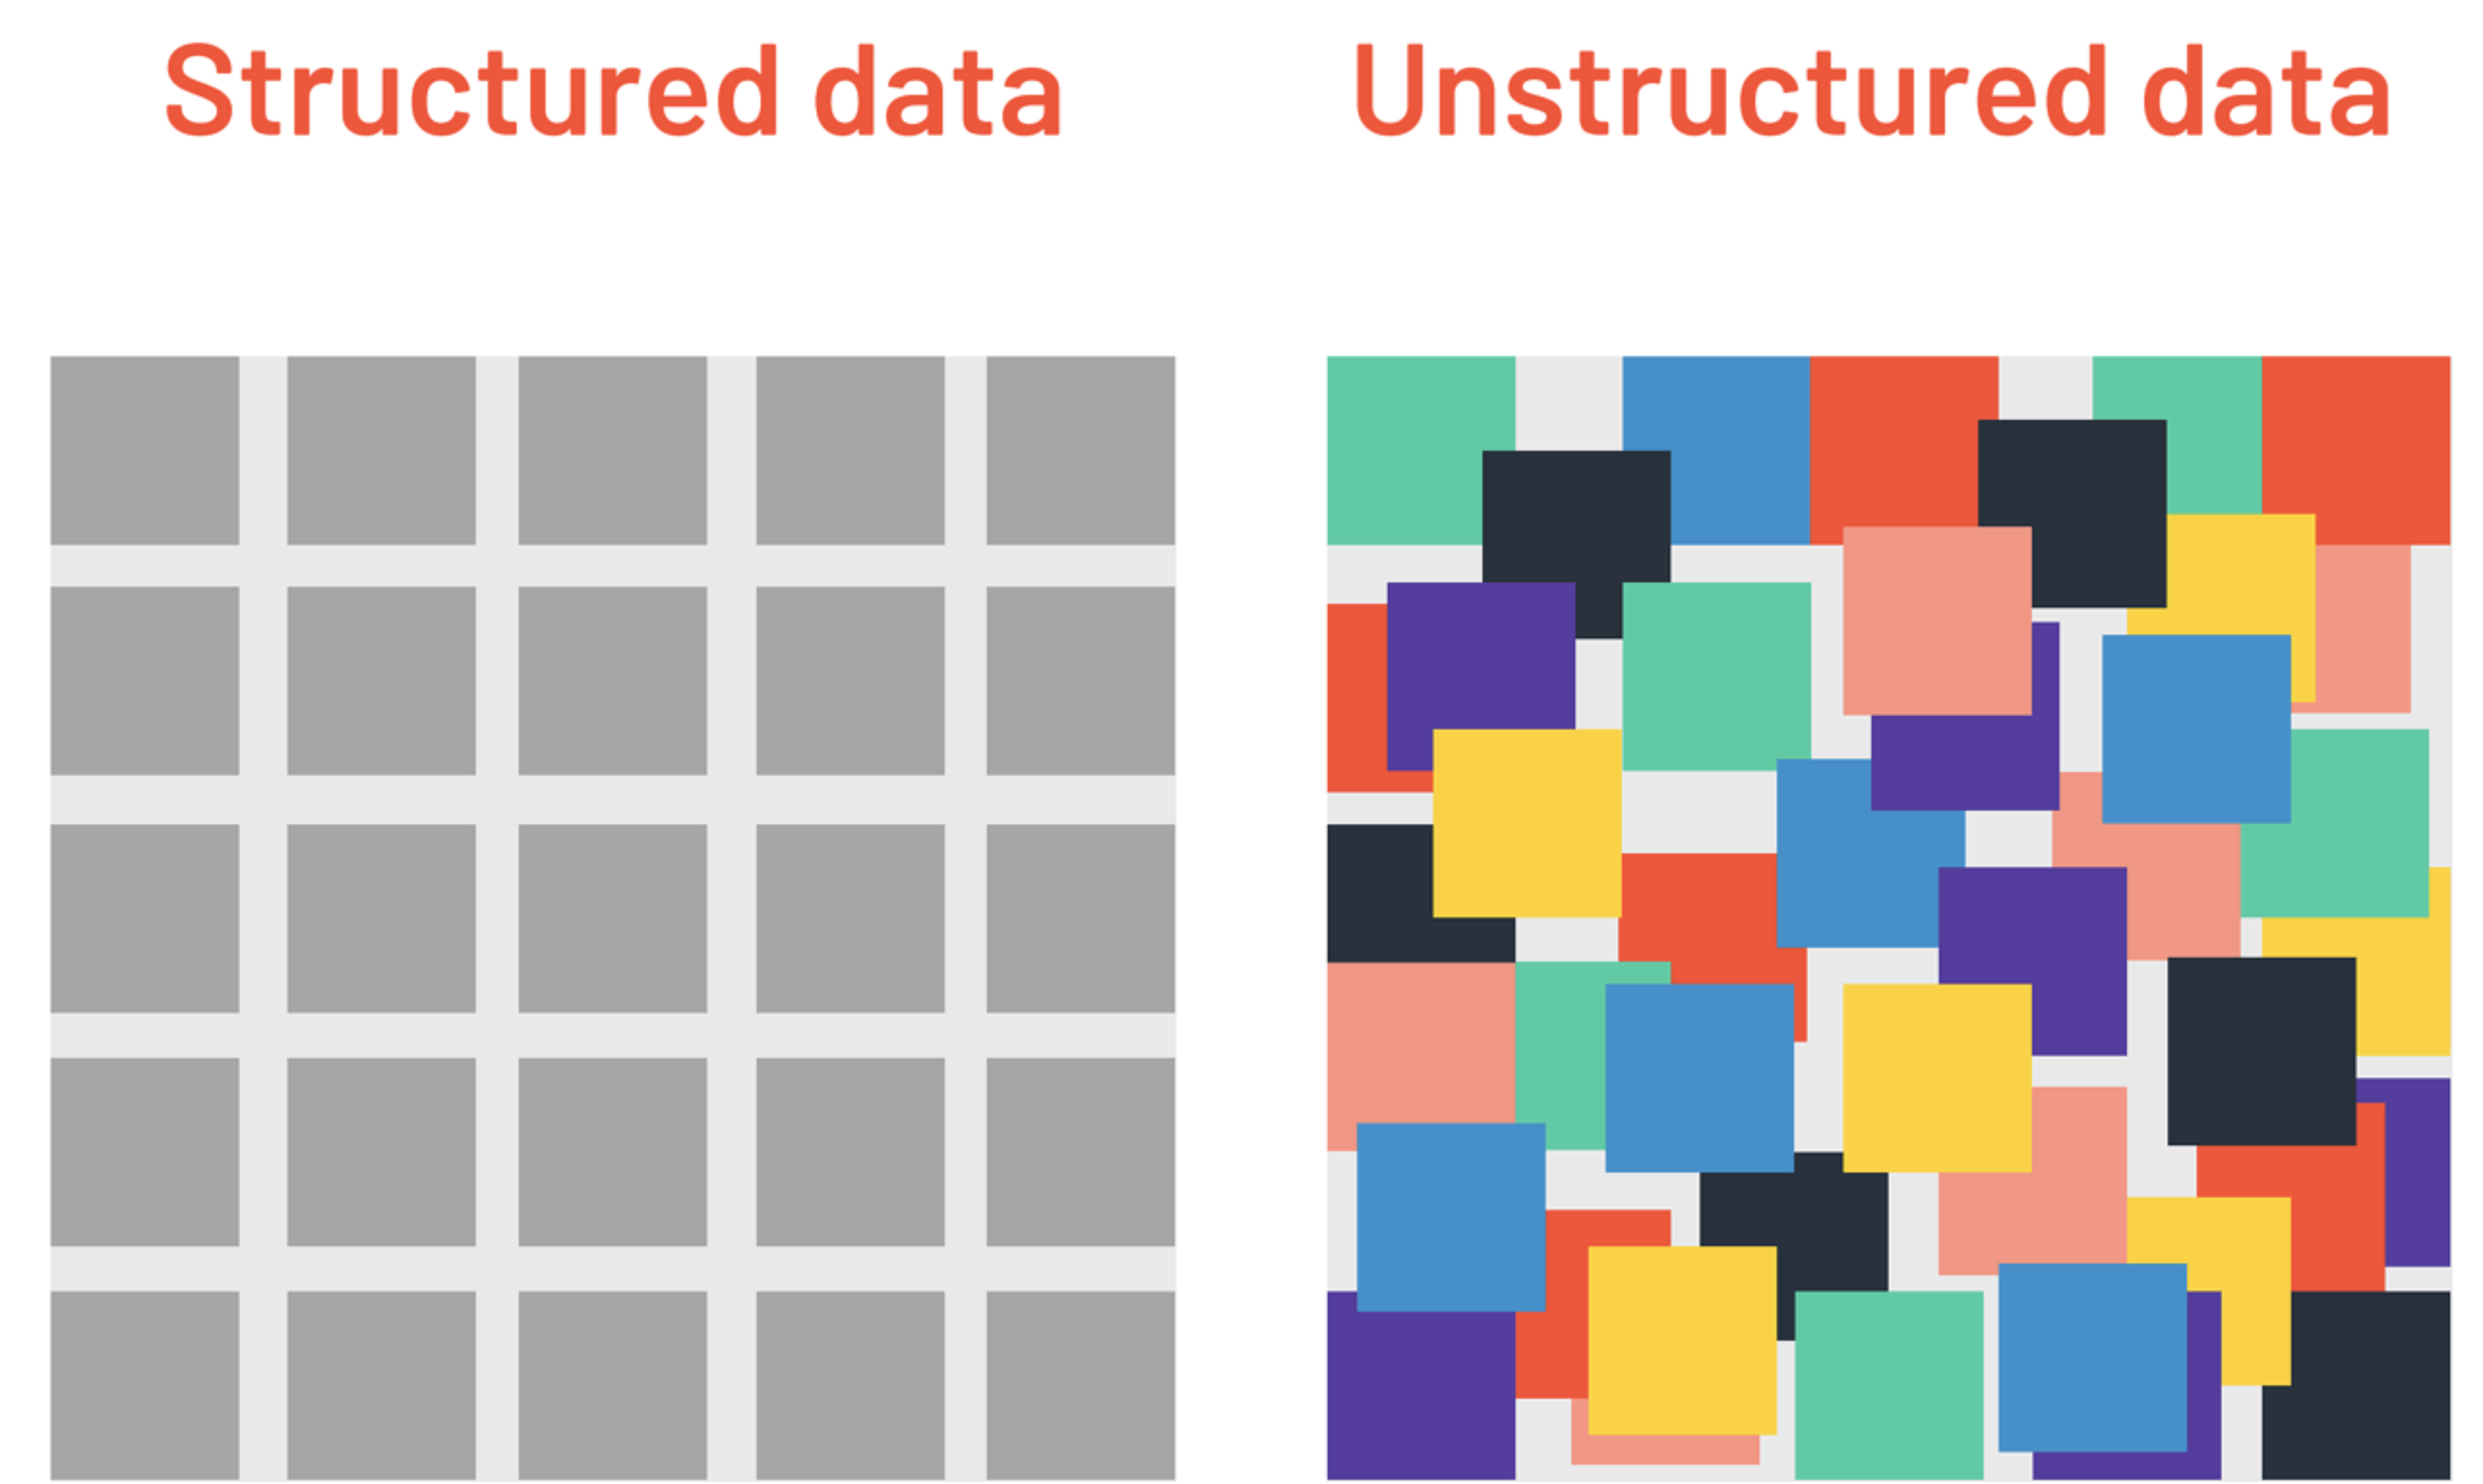
\includegraphics[scale=0.15]{src/ACT-3114/data-un-structured.png}
\end{center}

Types de variables:
\begin{description}
	\item[Quantitatives:]	Données numériques pouvant être:
		\begin{itemize}
		\item	Discrète, pour exemple des données de comptage; 
		\item	Continue, pour exemple des montants de sinistre.
		\end{itemize}
	\item[Qualitatives:]	Données catégorielles pouvant être:
		\begin{itemize}
		\item	Nominales, pour exemple le sexe; 
		\item	Ordinales, pour exemple des groupes d'âge.
		\end{itemize}
	\item[Temporelles]Données chronologiques représentant un état dans le temps;
		\begin{itemize}
		\item	Pour exemple, la quantité totale de pluie au Canada le 1er juillet 1990.
		\end{itemize}
	\item[Spatiales]	Données géographiques avec des coordonnées (pour exemple, la latitude et longitude).
\end{description}
\end{conceptgen}

\begin{algo2}[Conseils]
\begin{itemize}
	\item	Conserver un script séparé pour le traitement des données;
	\item	Documenter nos choix;
		\begin{itemize}
		\item	Si l'on omet quelques observations en raison de données aberrantes être conscient que ça peut biaiser les résultats.
		\end{itemize}
	\item	Effacer l'encre superflue 
	
	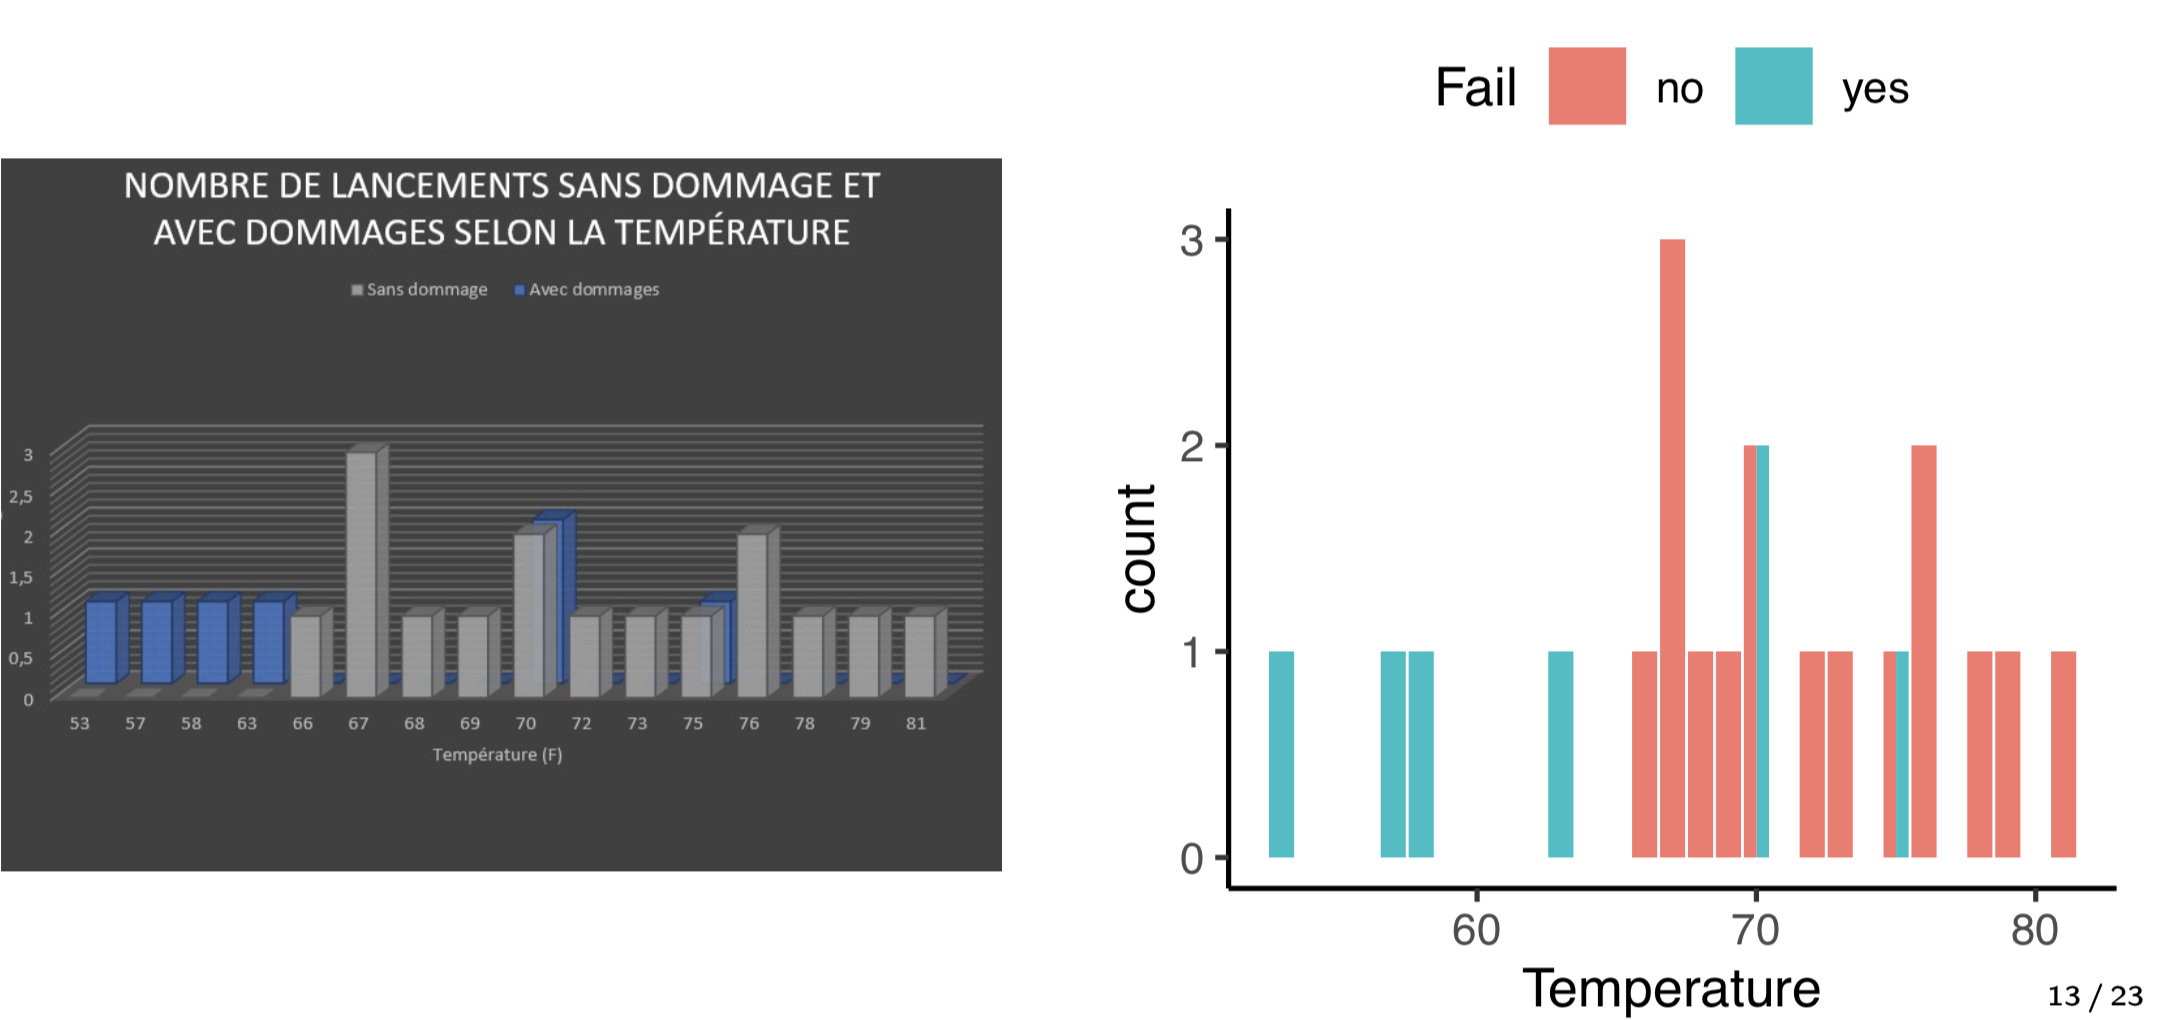
\includegraphics[scale=0.15]{src/ACT-3114/data-superfluous.png}
	\item	Considérer l'étique:
		\begin{itemize}[leftmargin = *]
		\item	Avons-nous l'autorisation d'utiliser les données?
		\item[]	Pour exemple, les données ouvertes du gouvernement avec peu de restrictions;
		\item	Est-ce qu'il y a des considérations étiques à l'utilisation des données?
		\item[]	Pour exemple, Facebook qui utilise les données de façon immorale;
		\item	Est-ce qu'il y a des biais dans les données pouvant causer préjudice?
		\item[]	Pour exemple, des données avec un biais sexiste ou raciste, des données financées par une compagnie.
		\end{itemize}
\end{itemize}
\end{algo2}

\begin{conceptgen}{Biais}
\begin{description}
	\item[d'échantillonnage]	Lorsque les données d'entraînement ne représentent pas de façon représentative la vraie population.\\
		Pour exemple:
		\begin{itemize}[leftmargin = *]
		\item	Entraîner une voiture autonome seulement le jour alors qu'elles peuvent être conduites jour et soir;
		\item	Sonder les lecteurs du Devoir sur le parti pour lequel ils vont voter à l'élection et donc ignorer ceux ne lisant pas le journal.
		\end{itemize}
	\item[de stéréotypes]	Données influencées par des stéréotypes (consciemment ou pas).\\
		Pour exemple:
		\begin{itemize}[leftmargin = *]
		\item	Entraîner un algorithme pour comprendre comment les personnes travaillent avec des images d'hommes sur des ordinateurs et de femmes à la maison;
		\item	L'algorithme aura tendance à penser que les hommes sont des programmeurs et les femmes des cuisinières.
		\end{itemize}
	\item[de mesure]	Données influencées par un problème avec l'instrument de mesure.\\
		Pour exemple:
		\begin{itemize}[leftmargin = *]
		\item	Entraîner un algorithme de reconnaissance d'image avec des images d'une caméra avec un filtre de couleur;
		\item	L'algorithme serait fondé sur des images ayant systématique mal-représentée le vrai environnement.
		\end{itemize}
	\item[de modèle]	Le compromis de biais-variance $B(\hat{\theta}) = \text{E}[\hat{\theta}] - \theta$.\\
		Pour exemple:
		\begin{itemize}[leftmargin = *]
		\item	Certaines variables ne sont pas considérées (ou mesurées);
		\item	Le modèle n'est pas assez flexible (compromis linéaire vs lisse)
		\end{itemize}
\end{description}
\end{conceptgen}

\section{Données manquantes}

Le chapitre utilise la \textbf{mise en contexte} suivante:
\begin{itemize}
	\item	Il y a une réclamation pour un accident d'auto en Ontario;
	\item	Le contrat d'assurance couvre les frais médicaux;
	\item	On désire calculer la probabilité de paiement (variable réponse) en fonction de:
		\begin{enumerate}
		\item	La gravité de l'accident (variable explicative);
		\item[]	3 niveaux: mineur-majeur-catastrophique;
		\item	La souffrance du réclamant;
		\item[]	Échelle de 1 (peu) à 5 (beaucoup);
		\end{enumerate}
\end{itemize}

\textbf{Problèmes} de modélisation:
\begin{itemize}
	\item	Comment analyser les données malgré les valeurs manquantes?
	\item	Quels enjeux ou problèmes devrait-on considérer dans la modélisation?
\end{itemize}

\subsection*{Terminologie}

\begin{definition}[Notation]
\begin{itemize}
	\item[$Y_{ij}$:] Valeur de la variable explicative $j$ pour l'observation $i$ où	$j \in \left\{ 1, \dots, p \right\}$ et $i \in \{1, \dots, n\}$;
	\item[$\matr{Y}_{n \times p}$:] Matrice contenant les données \textbf{complètes};
	\item[]	$\matr{Y}$ est partitionné en deux, $\matr{Y} = \left\{ \matr{Y}_{obs}, \matr{Y}_{mis} \right\}$
		\begin{itemize}
		\item[$\matr{Y}_{obs}$:] matrice avec les données ayant toutes les valeurs observées;
		\item[$\matr{Y}_{mis}$:] matrice avec les données comportant des valeurs manquantes;
		\end{itemize}
	\item[$\matr{R}_{n \times p}$:]	\textbf{Matrice de réponse} des variables indicatrices $R_{ij} = \matr{1}_{\{Y_{ij} \text{ observé}\}}$;
	\item[$\theta$:] \textbf{Paramètre de nuisance}
\end{itemize}
\end{definition}

\begin{examplebox}{Exemple de notation}
\begin{align*}
	\bm{Y}	
	&=	\begin{bmatrix}
		2	&	3	\\
		8	&	6	\\
		3	&	12	
		\end{bmatrix}	\\
	\bm{Y}_{obs}
	&=	\begin{bmatrix}
		2	&	.	\\
		8	&	6	\\
		.	&	.
		\end{bmatrix}	&
	\bm{Y}_{mis}
	&=	\begin{bmatrix}
		.	&	3	\\
		.	&	.	\\
		3	&	12	
		\end{bmatrix}	\\
	\bm{R}
	&=	\begin{bmatrix}
		1	&	0	\\
		1	&	1	\\
		0	&	0	
		\end{bmatrix}	
\end{align*}
\end{examplebox}

\subsection*{Mécanisme de non-réponse}
La distribution de $\matr{R}$ est le \textit{mécanisme de non-réponse};

\textbf{Types de données manquantes}:
\begin{enumerate}
	\item	\textbf{MCAR}: Missing Completely at Random;
		\begin{itemize}[leftmargin = *]
		\item	Le patron de non-réponse (pattern of missing values) est indépendant des données $\matr{Y}$;
		\item	Il s'ensuit que la probabilité de réponse $f(R | \matr{Y}, \theta)$ ne dépend pas des données complètes $\matr{Y}$:
			\begin{align*}
			f(R | \matr{Y}, \theta) &= f(R | \theta) \\
			\end{align*}
%		\item	Pour example
		\begin{examplebox}{Exemple avec un $\theta$ de 10\%}
		On perd $10\%$ des valeurs mesurées alors, $\forall i \in \{1, \dots, n\}, j \in \{1, \dots, p\}$, la distribution du mécanisme de non-réponse:
		\setlength{\mathindent}{-1cm}
			\begin{align*}
			R_{ij} 
			&\sim 	\text{Bernoulli}(p = 1 - \theta =  90\%)
			\end{align*}
		\setlength{\mathindent}{1cm}
		\end{examplebox}
		\item	\textbf{Tester} la différence de moyennes:
		\end{itemize}	
		\setlength{\mathindent}{-2cm}
			\begin{align*}
			\mathcal{H}_{0}:
			&\left\{ p_{\text{Cat, mis}} - p_{\text{Cat, obs}} = 0 \right\} 
			\text{et}	\\
			&\left\{ p_{\text{Maj, mis}} - p_{\text{Maj, obs}} = 0 \right\}
			\end{align*}
		\setlength{\mathindent}{1cm}
		\begin{itemize}
		\item[]	Est équivalent à tester: 
		\end{itemize}	
		\setlength{\mathindent}{-2cm}
			\begin{align*}
			\mathcal{H}_{0}
			&:	\text{les données sont MCAR}
			\end{align*}
		\setlength{\mathindent}{1cm}
		\begin{itemize}
		\item[]	avec un test du khi-carré de Pearson;
		\item[]	C'est-à-dire que le test est équivalent mais \textbf{pas} le hypothèses.
		\end{itemize}	
\end{enumerate}
\begin{enumerate}
	\setcounter{enumi}{1}
	\item	\textbf{MAR}: Missing at Random;
	\item[]	Can think of it as Missing \textit{Conditionnaly} at Random;
		\begin{itemize}[leftmargin = *]
		\item	La probabilité de réponse $f(R | \bm{Y}1616, \theta)$ dépend seulement des variables qui ont été observées dans le jeu de données $\matr{Y}_{\text{obs}}$:
			\begin{align*}
			f(R | \matr{Y}, \theta) &= f(R | \matr{Y}_{\text{obs}}, \theta) 
			\end{align*}
		\item	Exemple de patients d'un hôpital: les données sont MAR lorsque la probabilité de non-réponse ne dépend pas de la qualité de vie sachant l'âge;
		\item	Le négatif est qu'il est impossible de tester que, sachat l'âge, la probabilité de non-réponse ne dépend pas de la qualité de vie;
		\item	Il est \textbf{inconcevable} d'avoir un test pour MAR.
		\end{itemize}
	\item	\textbf{NMAR}: Not Missing at Random;
		\begin{itemize}[leftmargin = *]
		\item	Le patron de non-réponse pour $\matr{Y}$ est relié à sa valeur et les variables observées;
		\item[]	Ce même si on conditionne sur les valeurs observées;
		\item	La probabilité de réponse $f(R | \matr{Y}, \theta)$ dépend également de $\matr{Y}_{\text{mis}}$ et ne peut pas être simplifiée;
		\item	Pour exemple, les patients malades ne répondent pas aux sondages en plus des patients plus jeunes et donc la probabilité de réponse dépend de la qualité de vie;
		\item	Pour exemple, la probabilité de réponse dépend d'une autre variable non observée;
		\end{itemize}
\end{enumerate}

Visuellement on peut comparer les 3 patrons de non-réponse:
\begin{itemize}
	\item	On observe (MCAR) que la variable \textit{indépendante} $S$ ne dépend pas du patron de non-réponse $R$;
	\item	On observe (MAR) que $G$ influe la variable réponse $S$ et le patron de non-réponse $R$;
	\item	On observe (NMAR) qu'il y a un lien direct entre $S$ et $R$;
	\item	En dernier, puisque $Z$ n'est pas mesuré et que $Y$ y dépend c'est NMAR.
\end{itemize}
\textbf{Principe d'inclusion}: Si une variable est exclue cela peut créer une corrélation entre la variable indépendante $S$ et le patron de non-réponse $R$. De plus, ça peut changer le patron lui-même!

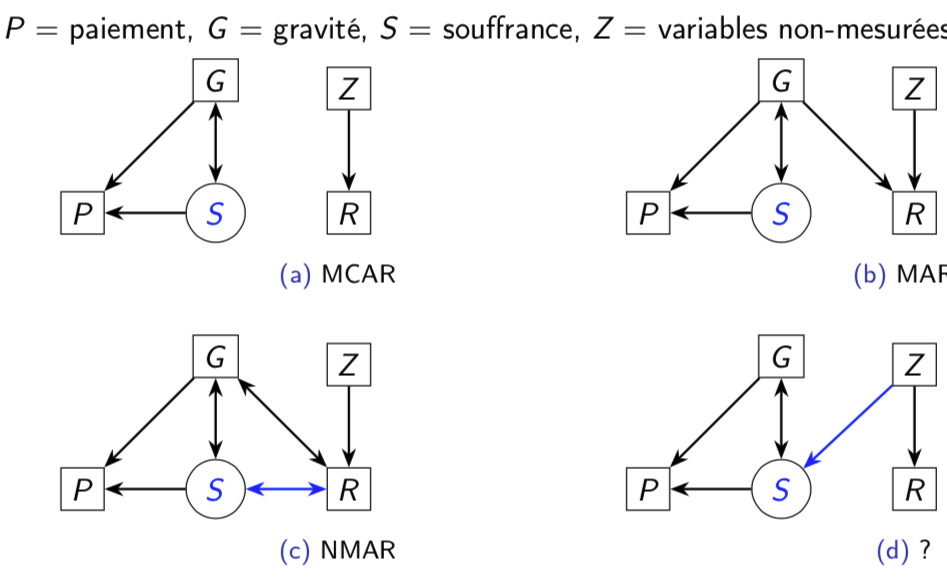
\includegraphics[scale=0.2]{src/ACT-3114/data-schema-missing.png}

Pour exemple, si on cherchait à supprimer des valeurs d'une BD:
\begin{description}
	\item[MCAR]	supprime des valeurs aléatoirement;
	\item[MAR]	supprime 60\% des valeurs pour les femmes et 40 \% des valeurs pour les hommes;
	\item[NMAR]	plus il y a de sinistres observés, plus il y a de chances que les valeurs soient manquantes.
\end{description}

Ordre de restriction des différents patrons
\begin{enumerate}
	\item	MCAR: plus \og restrictif \fg{} car les données doivent être manquantes complètement aléatoirement;
	\item[]	Même idée que l'hypothèse de normalité est restrictive puisque les données \textit{doivent} l'être \textbf{mais} cela nous permet d'utiliser plein de tests;
	\item[]	Comme une Bernoulli, il n'y a pas de paramètres;
	\item[]	plus restrictif alias moins flexible.
	\item	MAR: inclue les variables observées et donc il y a plus de paramètres;
	\item	NMAR: inclue toutes les variables et est donc le patron le plus flexible (alias, le moins restrictif).
\end{enumerate}

\subsection*{Visualisation et détection}
\begin{algo}{Traiter les données manquantes}
\begin{enumerate}
	\item	Détectez, visualisez et documentez les données manquantes;
	\item	Identifier le patron de non-réponse;
	\item[]	Pour exemple, voici quelques patrons de non-réponse pour quelques variables:

	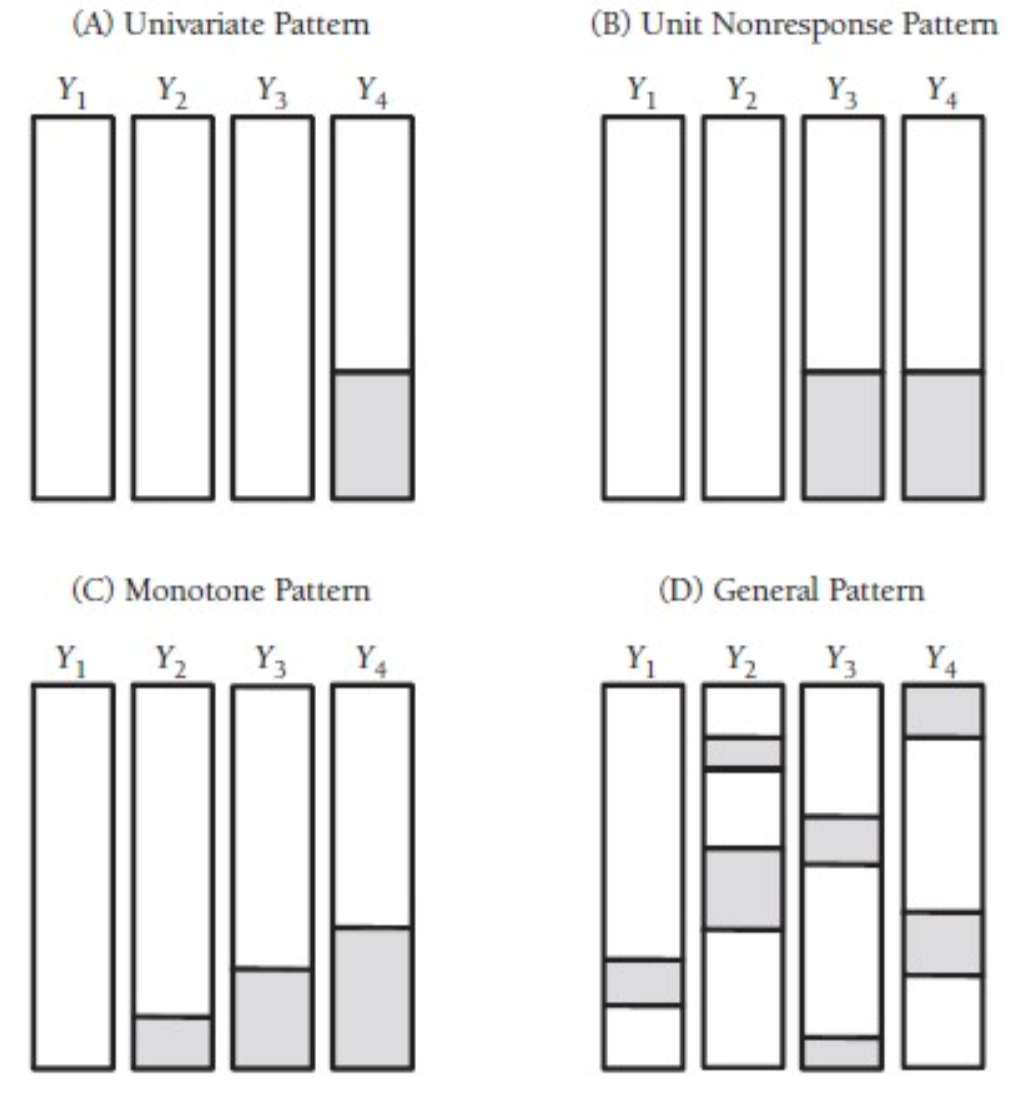
\includegraphics[scale=0.3]{src/ACT-3114/patrons-non-repoonse-exemples.png}
	\item[]	Exemple de patron univarié: concessionnaire ne pose jamais à ses assurés s'ils ont une piscine et donc la variable est manquante dans toutes ses données;
	\item	Comparer les distributions des autres variables selon la valeur des variables indicatrices $R_{1j}, \dots, R_{nj}$;
\end{enumerate}
\end{algo}

\subsection*{Identification des types de non-réponse}
\begin{itemize}
	\item	Pour les variables continues, on fait un \textbf{test $t$ sur les différences de moyenne} au lieu du khi-carré de Pearson comme pour MCAR;
	\item	Problème de comparaisons multiples;
	\item	Le test MCAR de Little est peu utile, mais peut adresser le problème de comparaisons multiple avec un hypothèse testant toutes les variables;
\end{itemize}

\subsection*{Traitement des données manquantes}

En continuant la mise en contexte, on suppose qu'on veut estimer le vecteur $\matr{\beta}$ des coefficients de la régression logistique pour prédire la probabilité de paiement;
Une question valide est si les options pour le traitement des données manquantes dépendent du \textbf{type} de non-réponse

\textbf{Options} de traitement:
\begin{enumerate}
	\item	Utiliser seulement les \textbf{cas complets} \textit{(complete-case analysis)};
		\begin{itemize}
		\item	L'option par défaut pour les fonctions :
			\begin{center}
			\texttt{lm, glm, na.rm, na.omit}
			\end{center}
		\item	\textbf{Impact}:
			\begin{itemize}
			\item[$\color{red}\downarrow$]	taille de l'échantillon	\\
			\item[$\color{red}\downarrow$]	taille de la corrélation des variables	\\
			\item[$\color{blue}\uparrow$]	variance des estimateurs	\\
			\item[$\color{red}\downarrow$]	puissance des tests	\\
			\end{itemize}
		\item	Uniquement valide sous \textcolor{ao(english)}{MCAR};
		\end{itemize}
	\item	Utiliser seulement les \textbf{cas disponibles} \textit{(available-case analysis)};
		\begin{itemize}
		\item	Utilise uniquement les données observées pour l'analyse;
		\item	Rarement applicable;
		\item	$\color{red}\downarrow$ la taille de l'échantillon \textbf{moins} qu'en utilisant d'uniquement les cas complets;
		\item	\textcolor{ao(english)}{Sans biais} \textbf{uniquement} sous \textcolor{ao(english)}{MCAR};
		\end{itemize}
	\item	\textbf{Imputation} simple par la \textbf{moyenne ou} la \textbf{médiane}
		\begin{itemize}
		\item	Substitue les \texttt{NA} par la moyenne ou médiane de la variable;
		\item	\textbf{Impact}:
			\begin{itemize}
			\item[$\color{red}\downarrow$]	variabilité de la variable	\\
			\item[$\color{red}\downarrow$]	corrélation de la variable avec les autres	\\
			\end{itemize}
		\item	Même sous MCAR, les données sont \textbf{sévèrement} \og distorted \fg{};
		\end{itemize}
	\item	Imputation simple par une régression;
		\begin{itemize}
		\item	Substitue les \texttt{NA} par la prévision d'une régression de la variable sur les autres avec les cas complets;
		\item	Si plusieurs variables ont des donnés manquantes, leurs patrons doivent être traités séparément;
		\item	L'inter \textbf{corrélation} des variables est \textbf{conservée}, mais est \textcolor{blue}{\textbf{surestimée}} (même si MCAR);
		\item	La variance est \textcolor{red}{\textbf{sous-estimée}}, mais \textbf{moins} qu'avec l'imputation par la moyenne;
%%%	-------------------------------
%%%	NOTE:
%%%	+	See if I can change the format for this to be arrows like the rest once 
%%%		I have a better understanding of whether I should make a distinction 
%%%		between "sous-estimé" and "diminution";
%%%	-------------------------------
		\end{itemize}
	\item	Imputation stochastique par une régression;
		\begin{itemize}
		\item	Ajoute un terme d'erreur $\varepsilon$ (normalement distribué) à la prévision de la régression;
%%%	-------------------------------
%%%	NOTE:
%%%	+	Je ne comprends pas ce que ça veut dire "dans un patron";
%%%	+	Pensais que patron c'était une pattern alors comment plusieurs variables pourraient être manquantes dans un patron?
%%%	-------------------------------
		\item	\textit{Si plusieurs variables sont manquantes dans un patron, les erreurs sont corrélées}
		\item	Corrige les biais pour la méthode d'imputation par la régression (sous-estimation de la variance et surestimation de l'inter corrélation des variables);
%%%	-------------------------------
%%%	NOTE:
%%%	+	Je ne comprends pas ce qu'on veut dire par "dans les calculs";
%%%	+	En tenir compte implique faire quoi?
%%%	+	Faire un ajustement en calculant le biais?
%%%	-------------------------------
		\item	La variance des paramètres est \textcolor{red}{\textbf{sous-estimée}}, \textit{sauf si on en tient compte dans les calculs};
		\item	Fonctions \texttt{R} utiles du paquetage \texttt{mice}:
			\begin{center}
			\texttt{mice.impute.norm.nob(), mice.impute.norm()}
			\end{center}
		\end{itemize}
	\item	Imputation simple \textit{hot-deck};
		\begin{itemize}
		\item	Substitue les valeurs \texttt{NA} d'une observation par les valeurs observées d'une autre observation choisie aléatoirement;;
		\item	Habituellement, cette observation fait parmi d'un sous-ensemble d'observations \textit{proches} (pensez au $K$-NN, clustering, etc.);
		\item	Souvent utilisée pour les sondages;
%%%	-------------------------------
%%%	NOTE:
%%%	+	Pourquoi ça ne les altère pas?
%%%	+	Puisqu'il aurait seulement le patron par observation et donc elle ne serait aucunement reliée à une autre observation?
%%%	-------------------------------
		\item	N'altère par les distributions univariées
		\item	$\color{red}\downarrow$	l'inter corrélation des variables;
		\item	Biais des estimations des coefficients $\matr{\beta}$ de régression;
		\end{itemize}
	\item	Imputation \textbf{multiple};
		\begin{itemize}
		\item	Répète l'imputation stochastique et agrège les résultats;
%%%	-------------------------------
%%%	NOTE:
%%%	+	Est-ce que "non biaisée" est vraiment équivalent à "estime correctement"?
%%%	+	Je pose que oui;
%%%	-------------------------------
		\item	Ce faisant, la variabilité additionnelle dût à l'imputation des valeurs manquante est adressée et la variance des estimateurs est \textit{non biaisée};
		\end{itemize}
\end{enumerate}

Autres méthodes:
\begin{itemize}
	\item	MLE avec données manquantes;
	\item	Algorithme EM (expectation-maximisation)
	\item	Inférence bayésienne;
\end{itemize}

\subsection*{Conseils}
\begin{itemize}
	\item	Conserver un script pour le traitement de données manquantes et ne \textbf{pas hard-coder};
	\item	\textit{Utiliser une méthode d'imputation qui respecte le format de la variable;}
	\item	Plus la proportion de non-réponses est élevée, plus l'impact sur l'analyse sera important;
	\item	S'il y a plusieurs patrons de non-réponse différents, l'ordre dans lequel les données sont imputées est important;
\end{itemize}

\end{multicols*}
%% -----------------------------
%% Fin du document
%% -----------------------------
\end{document}
